\documentclass[10pt,11pt,12pt,oneside]{book}
\usepackage[utf8]{inputenc}
\usepackage[left=1.2in,right=1in,top=1in,bottom=.8in]{geometry}
\usepackage{datetime}
\usepackage{emptypage}
\usepackage{graphicx}
\usepackage{capt-of}
\usepackage{amsmath}
\usepackage{enumitem}
\usepackage{float}
\usepackage[nottoc,notlot,notlof]{tocbibind}
\usepackage[toc,page]{appendix}

\parindent=0in
\newtimeformat{monthyear}{\THEMONTH \THEYEAR}
\setcounter{chapter}{0}


\begin{document}
\cleardoublepage
\begin{titlepage}
    \begin{center}
        \includegraphics[width=1.5in]{addu_logo.pdf}\\
        \vspace{1cm}
        \huge{Computational Fact Checking Using Knowledge Graphs}\\
        \vspace{1.5in}
        \large{Lean Raphael Alfafara\\Jan Leryc Ibalio}\\
        \vspace{1.5in}
        \large{ATENEO DE DAVAO UNIVERSITY\\SCHOOL OF ARTS AND SCIENCES\\DAVAO CITY}\\
        \vspace{1in}
        OCTOBER 2018
    \end{center}
\end{titlepage}

\frontmatter
\chapter*{Abstract}
We are living in the information age. The advent of personal computers and smartphones have created a society based on knowledge, and it has made accessing information easier today more than ever. However, technology can also be a means of spreading misinformation. Thus, there is a need to fact check statements we read and publish online. This paper intends to tackle the fact checking problem using knowledge graphs, using data gathered from Wikipedia. The study was divided into three phases. The first phase was an ideological classification task, where three different transitive closure algorithms were tested to see how accurately they could determine how semantically similar two topics are. Metric transitive closure with TF-IDF + Cosine Similarity was found to be the most accurate of the three algorithms tested, and was used for the succeeding phases. The second phase involved fact checking factual statements. The last phase of the study compared the computational fact checking method to human fact checkers. Rank order correlation coefficients showed that there is a correlation between judgments of human fact checkers and the computational fact checking method, making the method feasible for a fact-checking tool.\\

General Terms: fact checking, knowledge graph\\
Additional Key Words and Phrases: graph, facts, transitive closure, semantic proximity

\tableofcontents{}
\listoffigures{}
\listoftables{}

\mainmatter
\chapter{Introduction}

	\section{Background of the Study}
		We are living in an increasingly interconnected world. Mass media technology provides convenient ways to access news, stories, and other information at any time. It is no question that mass media play an essential role in shaping an individual’s thoughts and opinions, particularly in areas where audiences do not possess direct knowledge or experience \cite{happer_philo_2013}.\\
		
		However, modern technology can also be a means of deception and misinformation. As it grew, the internet had become widespread with misinformation, fraud, and other falsities. It had been reported that false information spreads six times faster than true information \cite{vosoughi2018}. Since our decisions and thoughts are largely based on the information that we find online, it would be detrimental to us if these falsities hinder us. Therefore, it is imperative to verify the integrity of information one receives.\\
		
		An enormous volume of information is being generated every day, and it has always been difficult for human fact checkers to cope with this amount of data. To combat the advent of misinformation, it is necessary to develop and improve computational fact checking methods that distinguish truth from falsity.

	\section{Problem Statement}
		This study will assess the accuracy of computational fact checking methods using knowledge graphs. The specific problems of the study are as follows:
		\begin{enumerate}
			\item Which algorithm gives more accurate truth scores: metric or ultra-metric closure?
			\item Does the use of cosine similarity and TF-IDF improve fact checking accuracy?
			\item How is the accuracy of the created fact checker comparable to human fact checkers?
			\item Is the selected combination of algorithms feasible for a computational fact-check tool?
		\end{enumerate}
	
		
	\section{Objectives}
		The general objective of the study is to evaluate the accuracy and speed of different combinations of computational fact checking methods and to build a fact-checking tool. The study aims to combine the use of directed graphs and negative weights, coupled with existing fact checking methods, and compare its accuracy to human fact checkers. The specific objectives of the study are as follows:
		\begin{enumerate}
		    \item Compare the accuracy of using metric and ultra-metric closure for path evaluation.
		    \item Evaluate the accuracy of the knowledge graph using cosine similarity and TF-IDF.
		    \item Compare the accuracy of fact checking between human fact checkers and the computational fact checker.
		    \item Create a computational fact checker using the optimal computational fact checking algorithm tested.
		\end{enumerate}

	\section{Significance of the Study}
		 Helping both unknowing and educated people protect themselves against the dangers of misinformation is crucial because as human beings living in the information age, information is a part of daily life. Information we read and hear has a massive influence on how we think and make decisions \cite{DelVicario_2016}.\\[8pt]
		
		Students browse the internet every day, and most students in this age are generally not very keen at evaluating the news and other information they see online \cite{mcgrew2017challenge}. Now more than ever, students need help from professionals to make sure that the information that they read are authentic and factual. Providing a tool to fact check sources online can be the first step to helping students.\\
	
		Writers and researchers can also benefit from this study. They need to make sure that they are not contributing to the problem of misinformation or deception. Providing a tool for writers and researchers can help them verify the credibility and facticity of their work.
		
		A lot of research has already been done on traditional fact-checking, but currently, the computational fact checking scene is not yet well-established. Hence, this study can be one of the first steps in increasing awareness and improving research on this subject.\\
	
	\section{Scope and Limitations}
		The study will cover fact-checking in the English language only. To ensure the integrity and fairness of facts we will gather, we will only be collecting data from factual sources such as encyclopedia entries, and not from potentially biased and partial sources such as news articles.\\
		
		Due to the large amount of data this study will need, this study will use data from Wikipedia, queried through their open-source Wikipedia API.\\
		
		This study will only be able to cover facts related to real world entities (e.g. people, places, names, events, etc.), and will not be able to cover facts concerning dates or any kind of measurement, since measurements cannot appear as the subjects in a subject-predicate-object triple, and consequently, cannot be vertices in a knowledge graph.\\

\chapter{Review of Related Literature}
	\section{The Spread of Misinformation}
	The availability of user-provided content in online mass media facilitates the aggregation of people around common interests, worldviews, and narratives. However, the internet permits for the fast dissemination of rumors and misleading news that often provoke naïve social responses \cite{DelVicario_2016}. There is worldwide concern over misinformation on the internet and the possibility that it can influence political, economic, and social well-being.\\[8pt]
	
	To understand how false information spreads, Vosoughi et al. used a data set of rumor cascades on Twitter from 2006 to 2017. At least 126,000 rumors were spread by approximately 3 million people. False news reached more people than the truth; the top 1\% of false news cascades diffused to between 1000 and 100,000 people, whereas the truth rarely diffused to more than 1000 people. This is attributed to the degree of novelty and the emotional reactions of the recipients of false news. Contrary to belief, bots accelerate the spread of true and false news at the same rate. This implies that false news spreads more than the truth because humans, not bots, are more likely to spread it [2].
	
	\section{Fact Checking}
	
	Fact checking is the act of determining the correctness and accuracy of factual assertations in non-fictional text. This may be done before (ante hoc) or after (post hoc) the text has been published. Ante hoc fact-checking (fact checking before dissemination) aims to remove errors and allow text to proceed to dissemination (or to rejection if it fails confirmations or other criteria). Post hoc fact-checking is most often followed by a written report of inaccuracies, sometimes with a visual metric from the checking organization \cite{fellmeth_horwitz_2009}. The task of fact-checking includes any analysis that challenges a competing account \cite{graves_2016}.\\[8pt]
	
	Studies in post hoc fact checking showed that such efforts often result in changes in the behavior of both the speaker (making them more careful in their pronouncements) and of the listener or reader (making them more discerning about the factual accuracy of content) \cite{amazeen_2015}.
	
	\section{Natural Language Processing}
	
	Natural language processing is an area of computer science that deals with the interactions and processes between natural human language and computers. One of the subsets of natural language processing is the understanding of natural language, and the extraction of information \cite{bird2009natural}.\\
	
	\subsection{Information Extraction}
	Information extraction is the act of extracting structured information from unstructured or semi-structured data \cite{mooney2005mining}. This discipline has developed automatic methods, typically through statistical means, for indexing large document collections and classifying documents \cite{freitag2000machine}.\\[8pt]
	
	It is often referred to text data mining. However, it can also be substituted with text analytics which has roughly the same meaning. Text analytics is a set of machine learning, statistical, and linguistic techniques. These techniques model and structure the information content of textual sources such as investigation, research, and business intelligence \cite{sethgrimes}.\\
	
	\subsection{Relationship Extraction}
	One of the subtasks of information extraction is relationship extraction. A relation is a semantic connection between (at least) two entities \cite{orr_2013}. Relationship extraction deals with the detection and classification of semantic relationships between entities, with the directionality of the relationship considered \cite {chagoyen2006discovering}. The goal of relation extraction is to learn relations from unstructured natural language text \cite{orr_2013}.
	
	\subsection{Named-entity Recognition}
	    Named-entity recognition (NER) is a subtask of NLP which deals with classifying words or phrases in a text into categories (e.g., people, names of organization, places, etc.) \cite {nadeau2007survey}. NER systems that use linguistic grammar-based techniques, as well as statistical models such as machine learning, have been created. Manually-created grammar-based systems typically obtain better precision, but at the cost of lower recall and months of work by experienced computational linguists \cite {kapetanios2013natural}. Statistical NER systems typically require a large amount of manually annotated training data \cite {lin2009phrase}.
	
	\subsection{Subject-object-predcate Triple}
		Extracted facts using information extraction from text often take in the form of a subject-predicate-object triple (e.g., “Socrates,” “is a,” “person”), which are central in the building of knowledge graphs. Most fact extraction approaches gather fact candidates though logical rules, but face trade-offs between scalability and precision. Scalable fact extraction approaches are susceptible to noisy patterns which degrade precision, while approaches that use deep logical reasoning cannot cope with large-scale data \cite{nakashole2012automatic}.
		
	\subsection{Stemming and Lemmatization}
	
		\subsubsection{Lemmatization}
		In linguistics, lemmatization is the process of grouping together the inflected forms of a word with the goal of analyzing the group as a single item. This process is made possible given the word's dictionary form \cite{Mller2015}.\\
		
		In computational linguistics, it is the algorithmic process of determining the dictionary form of a word based on its intended meaning. The process entirely depends on correctly identifying the definition of a word in a sentence, and finding out if it's appropriate to use, as well as within the broader context surrounding that sentence \cite{Mller2015}.
		
		
		\subsubsection{Stemming}
		In linguistic morphology and information retrieval, stemming is the process of reducing inflected words to their word stem or root form, by systematically cutting down words using a set of rules \cite{lovins1968development}.
		 
		It is usually sufficient that related words can be traced back to the same stem, regardless of the stem in itself is valid. In other words, this means that the stem does not need to be identical to the morphological base form of the word \cite{lovins1968development}.
	
	\subsection{Cosine Similarity}
		Cosine similarity is a measure of similarity between two non-zero vectors of an inner product space that measures the cosine of the angle between them. This technique does not offer judgments for magnitude but orientation.  The cosine similarity is mainly used in positive space, where the outcome is neatly bounded in [0, 1]. Cosine Similarity was taken from the term "Direction Cosine." This concept is analogous to the cosine, which is unity (maximum value) when the segments subtend a zero angle and zero (uncorrelated) when the segments are perpendicular \cite{singhal2001modern}.\\
		
		High-dimensional positive spaces usually see the most uses for cosine similarity. The technique gives a useful measure of how similar two documents are likely to be regarding their subject matter \cite{singhal2001modern}.\\
		
		In the context of natural language processing, a document can be transformed into a matrix of TF-IDF features and then compared to another document, obtaining its cosine similarity \cite{huang}.
	
	\subsection{NLP Tools}
	
		\subsubsection{Natural Language Toolkit}
			The Natural Language Toolkit (NLTK) is an open-source suite of libraries for symbolic and statistical natural language processing in the English language, written in the Python programming language. It is intended to support research and teaching in natural language processing and includes various demonstrations and corpora [8]. NLTK processes raw strings and returns strings. Thus it is a string processing library \cite {aho_lam_sethi_ullman_2006}.
		
		\subsubsection{SpaCy}
			SpaCy is another open-source library for natural language processing, also written in the Python programming language. Unlike NLTK, which is used primarily for education and research purposes, SpaCy provides libraries for production usage. Also, unlike NLTK, SpaCy processes the input strings as objects, and performs NLP tasks in an object-oriented approach \cite {aho_lam_sethi_ullman_2006}.
	
	
	
	\section{Knowledge Base}
	Knowledge bases are stores of information which may be structured or unstructured. A knowledge base typically consists of facts and an inference engine, which reasons out those facts to deduce new facts or highlight inconsistencies \cite {scholl_2016}.\\
	
	Knowledge base construction (KBC) is the process of populating a knowledge base with facts (or assertions) extracted from text. Rule-based approaches to knowledge base construction rely on the observation that there are often a small number of rules that can achieve both high precision and high recall. For example, to identify mentions of people, the knowledge base performs string matching between the text and variations of a dictionary of person names (e.g., abbreviations and first/last name ordering). Because these dictionaries of variation types cover most variations, the knowledge base can achieve both high recall and high precision in knowledge base construction. \cite{hayes1983building},\cite{arasu2003extracting},\cite{mooney1999relational}.\\
	
	Statistical Machine Learning Approaches target KBC tasks that cannot be covered by a small set of deterministic rules. To address this issue, classical statistical approaches employ machine learning models such as logistic regression \cite {michelakis_krishnamurthy_haas_vaithyanathan_2009}, \cite{lafferty2001conditional} to learn model parameters from training examples, e.g., annotations of sentences that describe entity relationship.\\
	
	
	\section{Knowledge Graph}
	
	Facts extracted using various extraction techniques can take in the form of subject-predicate-object triples. One form of a knowledge base that makes use of interconnected subject-predicate-object triples are knowledge graphs. The graph’s nodes denote entities (i.e., the subject or objects of facts), and the graph’s edges denote predicates (which links the subject and the object together) \cite{sutton2004collective}.\\
	
	 An example of a knowledge graph in real-world applications is the Google Knowledge Graph. The Google search engine uses a knowledge graph to provide information to search queries, powered by Freebase \cite{goog_kg}, an online collection of structured data harvested from many sources, including individual, user-submitted wiki contributions \cite{freebase}.
	
	\subsection{Semantic Proximity from Transitive Closures}
	 It is possible to derive semantic proximity using transitive closures in complex networks such as knowledge graphs. The concept of transitive closure is important because it allows us to identify not only transitive cliques in a network but also indirectly related items \cite{SIMAS2015}.\\
	
	Transitive closure of a knowledge graph is an isomorphism between the graph and the proximity of nodes. These isomorphisms show how alternative distance/transitive closures impose distortions of the original network. It allows the computation of indirect associations in complex networks \cite{SIMAS2015}.
	
	\subsubsection{Metric Closure}
	Semantic proximity, and consequently, the truth value of a statement in a knowledge graph, can be computed using the metric transitive closure. The truth value $\tau(e) \in [0, 1]$ of a new statement $e = (s, p, o)$ can be derived from the transitive closure of the Wikipedia Knowledge Graph (WKG), by a function that maps the set of possible paths connecting $s$ and $o$ to a truth value $\tau$. Paths have the form $P_{s,o} = v_{1}, v_{2}\ldots v_{n}$, where $vi$  is an entity node (either $s$ or $o$ in a statement), and $n$ is the total number of nodes between $s$ and $o$. The generality of the entities (or in the case of graphs, the degree of a node) along a path can serve as a measure of its length. The edges in a statement can be aggregated to define a semantic proximity function:
	$$
	W(P_{s,o}) = W(v_{1}\ldots v_{n}) = {[1 +  \sum_{i=2}^{n-1} log k(v_{i})]}^{-1}
	$$[H]
	where $k(v)$ is the count of in-degrees of a single entity). A path length in a metric transitive closure network is computed by summing the distance weights in the path \cite{SIMAS2015}.
	
	\begin{figure}[H]
		\begin{center}
			\includegraphics[width=2in]{Obama_Islam.pdf}\\
			\label{fig_tc_obama}
			\caption{The shortest path returned by the metric closure function for the statement “Barack Obama is a Muslim.” The path traverses high-degree nodes representing more generic entities, such as Canada, and is assigned a low semantic proximity score. }
		\end{center}
	\end{figure}
	
	\subsubsection{Ultrametric closure}
	Aside from the metric transitive closure, alternative definitions of $\tau(e)$ can be used. One alternative definition uses a different optimization principle, widest bottleneck, also known as the ultrametric closure \cite{gruber1993translation}, which maps paths to the function:
	$$
	W(P_{s,o}) = W(v_{1}\ldots v_{n}) =\begin{cases}1 & n=2\\{[1+max^1_2 \{log k(v_{i})\}]^{-1}} & n>2\end{cases} 
	$$[H]
	
	 In the ultrametric closure, instead of path length being computed by summing the edges in a path (as in the metric closure), the path length is measured by the “weakest edge” in the path: the largest distance edge weight or the smallest proximity edge-weight \cite{SIMAS2015}.
	
	The ultrametric closure of a graph leads to a heavier distortion of the original network than what we get from the metric closure of the same graph. This method also leads the nodes of the graph to be closer in proximity. \cite{SIMAS2015}. 
	
	\subsection{Distortion of Metric vs. Ultrametric Closure}
	
	In the case of the metric closure, because the distance weight of every edge in a path is summed, there is a built-in penalty for the number of indirect edges in the path. This would lead to the metric transitive closure results in significantly fewer edges being altered in the original network; only those indirect paths comprised of a few edges, with every distance edge-weight relatively small, may
	provide a shorter indirect connection than the original direct connection. The metric closure imposes a weaker distortion of the original graph \cite{SIMAS2015}.
	
	\subsection{Generality of a Knowledge Graph Entity}
	In the context of knowledge graphs, the generality of a vertex is calculated using the frequency of the term associated with that vertex \cite{sutton2004collective}.\\
	
	In the field of information retrieval and text mining, term frequency is a numerical statistic that is used often as a weighting factor.  Suppose a set of English text documents is to be ranked based on its relevance to the query, "the brown cow". The first step is eliminating documents that do not contain all three words "the", "brown", and "cow”. To further distinguish the uneliminated results, the number of times a term occurs in a document can be counted. The weight of a term that occurs in a document is simply proportional to the term frequency \cite{lao2011random}.\\
	
	Another form of a weighting factor of terms is the term frequency-inverse document frequency, or tf-idf. The tf-idf value is proportional to the number of times a word appears in the document and is offset by the frequency of the word in the corpus. This helps account for the fact that some words with low weight might appear more frequently than more meaningful words \cite{luhn19571}.
	
	\section{Graph Data Structure}
	\subsection{Adjacency List}
	An adjacency list representation of a graph consists of a list Adj of size $|V|$, one for each vertex in $V$. For each $u \in V$, the adjacency list Adj[u] contains all the vertices $v$ such that there is an edge $(u, v) \in E$. Alternatively, $Adj[u]$ may also contain references or pointers to vertices where an edge $(u, v) \in E$ exists. This representation is best suited for sparse graphs, where the cardinality of the edges $|E|$ is much less than the $|V|2$ (the maximum number of edges a graph may have). Adjacency list representations can easily be adapted to represent weighted graphs \cite{beel2016paper}.\\
	
	\begin{figure}[!htb]
		\centering
		\includegraphics[height = 2in]{Figure_2.pdf}
		\caption{A visual representation of an adjacency list (right) for the graph (left).}
		\label{fig:adjacency_list}
	\end{figure}
	
	One of the disadvantages of the adjacency list representation is that does not provide a way to determine whether a given edge $(u, v)$ exists in the graph, other than to search for $v$ in the adjacency list $Adj[u]$ \cite{beel2016paper}.
	
	\subsection{Adjacency Matrix}
	In an adjacency matrix representation of a graph, we assume that each of the vertices are numbered in an arbitrary manner. The adjacency matrix representation consists of a $|V| \times |V|$ matrix $A = (a_{ij})$ such that \cite{beel2016paper}:\\
	
	----------<Formula>-----------\\
	Adjacency matrix representations of graphs require  $\theta(V^{2})$ memory. This implies memory required to represent an adjacency matrix graph is always $\theta(V^{2})$ regardless of the number of edges in the graph, since each edge, existent and nonexistent, is represented by a $1$ and $0$ respectively. Like the adjacency list representation, adjacency matrices can also easily adapt weight values, by storing the weight value in $a_ij$ instead of $0$s and $1$s. Nonexistent edges can be represented by a nil value. The adjacency matrix representation is suited for a dense graph, in which $|E|$ is close or equal to $|V|^{2}$. \cite{beel2016paper}.\\
	
	\begin{figure}[!htb]
		\centering
		\includegraphics[height = 2in]{Figure_3.pdf}
		\caption{. A visual representation of an adjacency matrix (right) for the graph (left).}
		\label{fig:adjacency_matrix}
	\end{figure}
	
	\subsection{Graph Searching Algorithms}
	\subsubsection{Breadth-first Search}
	Breadth-first search is one of the simplest searching algorithms for a graph and is crucial for many important graph algorithms such as Prim’s minimum spanning tree algorithm and Dijkstra’s single-source shortest path algorithm \cite{beel2016paper}. Pseudocode for a breadth-first search follows:\\
	
	Given a graph $G = (V, E)$ and a source vertex $s$, a breadth-first search is done by systematically exploring all the edges that are reachable from s. It discovers all vertices at distance k from s before discovering vertices at distance greater than k+1. It can be adjusted to compute the distance (smallest number of edges) from $s$ to each reachable vertex. It also produces a breadth-first tree that contains a tree of discovered vertices with s as the root. This algorithm works on both directed and undirected graphs \cite{beel2016paper}. 
	
	\subsubsection{Depth-first Search}
	One algorithm for searching/traversing through a graph is the depth-first search. It traverses a graph as deep as possible before backtracking \cite{beel2016paper}. Pseudocode for a recursive depth-first search follows:\\
	
	A depth-first search explores edges out of the most recently discovered vertex $v$ that still has unexplored edges leaving it. Once all of $v$’s edges have been explored, the search backtracks to explore edges leaving the vertex from which v was discovered. This process of searching “deeper” in the graph whenever possible continues until all vertices that are reachable from the original source vertex have been discovered. If there are any undiscovered vertices remaining, one of those undiscovered vertices are arbitrarily selected to be the new source. The search process is repeated until all vertices have been discovered \cite{beel2016paper}. 
	
	\subsection{Shortest Path Algorithms}
	Given a graph $G = (V, E)$, the goal of single-source shortest path algorithms is to find the shortest path from a given source vertex $s \in V$  to each vertex $v \in V$.  Single-source shortest path algorithms can be adapted to other variants of the shortest path problem, namely single-destination shortest-paths, single-pair shortest-paths, and all-pairs shortest-paths \cite{beel2016paper}.
	
	Single-destination shortest-path algorithms aim to find the shortest path to a given destination vertex t from each vertex $v$. By reversing the direction of each edge in the graph, the problem can be reduced to a single-source problem. Single-pair shortest-path algorithms aim to find the shortest path from u to v for given vertices $u$ and $v$. All-pairs shortest-paths algorithm aim to find the shortest path from $u$ to $v$ for every pair of vertices $u$ and $v$ \cite{beel2016paper}. 
	
	\subsubsection{Dijkstra's Algorithm}
	One example of a shortest-path algorithm is Dijkstra’s algorithm, developed by Dutch computer scientist Edsger W. Dijkstra in 1956. It finds the shortest path between a vertex and every other vertex in the graph. Hence, it solves single-source shortest path problems \cite{cormen_leiserson_rivest_stein_2009}. 
	Pseudocode for Dijkstra’s algorithm follows:\\
	
	The algorithm follows the following steps:\\
	\begin{itemize}
		\item {Mark all vertices as unvisited. Create a set of unvisited vertices}
		\item {Assign tentative distance values for all the unvisited nodes: zero for the source vertex and infinity for all other vertices. Set the source vertex as the current vertex.}
		\item {Calculate all the tentative distances of all unvisited neighbors of the current vertex. Compare the new tentative distance to the current value assigned and reassign the smaller value.}
		\item {Mark the current vertex as visited and remove it from the set of unvisited vertices.}
		\item {If the destination vertex has already been visited, the algorithm has finished. Otherwise, the unvisited node that has the smallest distance value is marked as the current vertex and the third step is repeated, until the destination vertex is visited. }
	\end{itemize}
	
	Dijkstra’s algorithm is based on the principle of relaxation, in which an approximation to the correct distance is gradually replaced until an optimal solution is reached. Dijkstra’s algorithm is faster than the Bellman-Ford algorithm but lacks the capability to handle negative weights. An extended version of Dijkstra’s algorithm is the A* (a-star) algorithm \cite{mehlhorn2008algorithms}, [35]. 
	
	\subsubsection{Bellman-Ford Algorithm}
	The Bellman–Ford algorithm is an algorithm that computes shortest paths from a single source vertex to all of the other vertices in a weighted graph with negative weights algorithm (single-source shortest path problem with negative weights) [36]. Pseudocode for the Bellman-Ford algorithm follows:\\
	
	Similar to the Dijkstra’s algorithm, the principle is relaxation is used in the Bellman-Ford algorithm. However, Dijkstra’s algorithm makes use of a priority queue to select the closest vertex that has not been processed yet and performs the relaxation process on the current vertex’s outgoing edges, while the Bellman-Ford algorithm relaxes all edges $|V|$— 1 times.
	
	\subsubsection{Floyd-Warshall Algorithm}
	The Floyd-Warshall algorithm is an algorithm for finding the shortest sum of weights between all pairs of vertices. Unlike Dijkstra’s algorithm and the Bellman-Ford algorithm, this algorithm solves the all-pairs shortest path problem (i.e. finding all distances between all pairs of vertices). This algorithm was developed independently from each other by Floyd (1962) and Warshall (1962). This algorithm can be extended to or modified in order to find the transitive closure of a graph, or the widest paths between all pairs of nodes in a weighted graph \cite{beel2016paper}. 
	
	\subsection{Minimum Spanning Tree}
	A minimum spanning tree is a subset of the edges of a connected, edge-weighted graph that connects all vertices together, without cycles and with the minimum possible total edge weight. That is, it is a spanning tree whose sum of edge weights is as small as possible. More generally, any edge-weighted undirected graph (not necessarily connected) has a minimum spanning forest, which is a union of the minimum spanning trees for its connected components. The number of edges in a minimum spanning tree of a graph $G$ is $|G.V| - 1$. There may be several minimum spanning trees of the same weight; in particular, if all the edge weights of a given graph are the same, then every spanning tree of that graph is minimum. If all the weights are distinct for each edge, then there will only be one unique minimum spanning tree. More generally, if the edge weights are not all distinct then only the set of weights in minimum spanning trees is certain to be unique; it is the same for all minimum spanning trees \cite{bang2008digraphs}.\\
	
	\begin{figure}[!htb]
		\centering
		\includegraphics[height = 2in]{Figure_4.pdf}
		\caption{A planar graph and its minimum spanning tree. Each edge is labelled according to its weight, and its length is proportional to its weight.}
		\label{fig:my_label}
	\end{figure}
	
	One of the properties of a minimum spanning tree is the cut property. For any cut $C$ of the graph, if the weight of an edge e in the cut-set of $C$ is strictly smaller than the weights of all other edges of the cut-set of $C$, then this edge belongs to all MSTs of the graph \cite{bang2008digraphs}.\\
	The first algorithm for finding the minimum spanning tree of a graph was developed in 1926 by Czech scientist Otakar Borůvka. Borůvka’s algorithm proceeds in a sequence of stages. In each stage, a forest F consisting of the minimum-weight edge incident to each vertex in the graph is identified, then forms the graph $G1 = G/F$ as the input to the next step. Here $G/F$ denotes the graph derived from G by contracting edges in F. By the cut property, these edges belong to the minimum spanning tree of the graph. Each Borůvka step takes linear time. Since the number of vertices is reduced by at least half in each step, Borůvka algorithm takes $O(m log n)$ time \cite{bang2008digraphs}.\\
	
	
	
	
	
	
	
	
	
	
	
	
	
	
	
	
	
	
	
	\section{Datasets}
	 
	\subsection{The DBpedia Project}
	One of the sources of data that will be used is this study is the DBpedia dataset. DBpedia (dbpedia.org) is a project created by the Free University of Berlin and Leipzig University aiming to extract content from the information created in the Wikipedia project. This information is made available under free licenses on the world wide web, allowing others to reuse their work (CC-BY-SA) \cite{ciampaglia2015computational}. DBpedia allows users to semantically query relationships and properties of Wikipedia resources, including links to other related datasets \cite{dbpedia}.\\[8pt]
	The DBpedia data set describes 4.58 million entities, out of which 4.22 million are in a consistent ontology, including 1,445,000 persons, 735,000 places, 123,000 music albums, 87,000 films, 19,000 video games, 241,000 organizations, 251,000 species and 6,000 diseases. DBpedia uses the Resource Description Framework (RDF) to represent extracted information and consists of 3 billion RDF triples, of which 580 million were extracted from the English edition of Wikipedia and 2.46 billion from other language editions \cite{dbpedia}.
	
	\subsection{RDF}
	RDF is a family of World Wide Web Consortium (W3C) specifications originally designed as a data model for metadata. It has come to be used as a general method for conceptual description or modeling of information that is implemented in web resources \cite{dbpedia}. It is the preferred format of the DBpedia datasets.\\[8pt]
	One of the datasets in the DBpedia project is the DBpedia ontology. It was used by \cite{sutton2004collective} in their knowledge graph to recreate the full ontological hierarchy of the graph. The ontology divides and separates variables that are to be used in a certain set of computation and establishes the relationship between said variables \cite{bikakis_tsinaraki_gioldasis_stavrakantonakis}.
	
	\subsection{Google Relation Extraction Corpus}
	The Google Relation Extraction Corpus (GREC) is a dataset by Google containing human-judged statements about public figures, with nearly ten thousand statements containing “place of birth” and over forty thousand statements containing “attended or graduated from an institution”. Each of these statements are judged by at least five raters, and can be used on different applications (e.g. train or evaluate relation extraction systems) \cite{orr_2013}.\\[8pt]
	
	Each relation is in the form of a triple: the relation in question, called a predicate; the subject of the relation; and the object of the relation. In the relation “Stephen Hawking graduated from Oxford,” Stephen Hawking is the subject, graduated from is the relation, and Oxford University is the object \cite{orr_2013}. 
	
	
	\section{Term Frequency - Inverse Document Frequency}
	TF-IDF is a statistic to measure term frequency while also reflecting how important a word is in a document in a corpus. TF-IDF is commonly used as a weighing factor in information retrieval and text mining \cite{skiena1998algorithm}.  The TF-IDF value increases proportionally to the number of times a word appears in a document. It is offset by the word’s frequency in the data set, which adjusts for the fact that some words appear more frequently without adding value to the document (such as stop words). 83\% of text-based recommender systems use TF-IDF [40].
	
	\section{k-Nearest Neighbors Algorithm}
	The k-nearest-neighbors algorithm (often abbreviated as k-NN) is a non-parametric method that is used for classification. The output of a k-NN classification is a class membership. The class membership is determined by a positive integer $k$ (typically a small integer). If $k = 1$, an object’s membership is simply assigned to the class of the nearest neighbor. The k-NN algorithm is an example of instance-based learning (also called lazy learning).
	
	\section{Support Vector Machines}
	Support vector machine are supervised learning models used for classification or regression. A model is built from training examples, and classifies new examples into either of the two classes. An SVM model is a representation of data in space, mapped in such a way that would maximize the gap between the two classses. In addition to separating the classes linearly, SVMs can perform non-linear separation by mapping the data into a higher dimension space (otherwise known as kernel tricks) \cite{Cortes1995}. 
	
	
	\section{Theoretical Framework}
	
	The following framework is based on the paper on computational fact checking by \cite{ciampaglia2015computational}. To obtain the knowledge graph, RDF triples were downloaded from the DBPedia project (dbpedia.org). Three datasets were used to build the knowledge graph: the “Types” dataset, which contains triples in the form (subject, “is-a”, class), where class is a category of the DBpedia ontology; the “Properties” dataset, which contains triples obtained from Wikipedia infoboxes (a template Wikipedia uses to present a subset of information about its subject); and the DBpedia ontology, which contains triples in the form (subject, “subclass-of”, object). This third dataset was used to reconstruct the full ontological hierarchy of the graph.\\
	
	The predicate parts of all triples were discarded (since the study utilizes an undirected WKG), and all triples having the same subject and object were conflated, obtaining an edge list. In this process, triples whose subject or object belonged to external namespaces (e.g. FOAF and schema.org) were discarded. The entities were then used as vertices in the knowledge graph. The degrees of the vertices were then computed, obtaining a complete knowledge graph.\\
	
	\subsection{Ideologial Classification of the US Congress}
	
	The knowledge graph was used to classify members of the US Congress into Democratic and Republic members, using the ideologies they endorse as criteria. Entities listed in the ontology by means of a statement ($Y$, “is-a”, “Ideology) were considered, to obtain a list of ideologies.\\
	
	For every politician $X$ and ideology $Y$, the truth value of the statement “$X$ endorses ideology $Y$.” was calculated, and a feature matrix was obtained. To perform the classification, two off-the-shelf classifier algorithms were used: k-Nearest Neighbors and Random Forests. To assess the classification accuracy, the study obtained the F-score of the classification and teh area under the receiver operating characteristic (ROC) curve, using 10-fold cross-validation.\\
	
	\subsection{Simple Factual Statements}
	Simple factual statements were formed by combining $N$ subject entities with each N object entities. The procedure was performed in four subject areas: Academy Awards for Best Movie, US presidential couples, US states, and world capitals. All data were taken from Wikipedia. Triples indicating a true statement  already present in the knowledge graph were removed, to make the tests unbiased.
	
	\subsection{Independent Corpus of Statements}
	The second ground truth dataset was based on Google Relation Extraction Corpus (GREC), which contains subject-predicate-object triples, with judgments given by five human annotators. For simplicity, the study focused on two types of statements, about education degrees, and institutional affiliations. 
	
	For each statement in the GREC, their respective ratings were mapped into an ordinal scale between +5 (all raters replied 'No') and +5 (all raters replied 'Yes') and compare them to the truth values computed by the computational fact checker. Similar to the previous task, statements already present in the knowledge graph were removed before computing the truth values.
	
	\begin{figure}
	    \centering
	    \includegraphics[width=\textwidth,height=\textheight,keepaspectratio]{theoretical_framework.pdf}
	    \caption{Theoretical Framework}
	    \label{fig:theoretical_framework}
	\end{figure}




%------------------------------------------------------------------------------------
%    CHAPTER 3 - METHODOLOGY
%------------------------------------------------------------------------------------


\chapter{Research Design and Methodology}

\begin{figure}
	\centering
	\includegraphics[width=\textwidth,height=900pt,keepaspectratio]{conceptual_framework.pdf}
	\caption{Conceptual Framework}
	\label{fig:conceptual_framework}
\end{figure}
\clearpage



\section{Methodology}
The study will have three phases. The phases will be as follows:


\begin{enumerate}[label*=\arabic*.]
	
	\item {Ideological Classification Task} 
	\begin{enumerate}[label*=\arabic*.]
		\item Data gathering and preprocessing
		\item Path matrix calculation
		\item Page data querying and caching
		\item Truth value matrix calculation
		\item Classification and evaluation
	\end{enumerate}

	\item {Validation on Simple Factual Data}
	\begin{enumerate}[label*=\arabic*.]
		\item Data gathering and preprocessing
		\item Path matrix calculation
		\item Page data querying and caching
		\item Truth value matrix calculation
		\item Evaluation of Accuracy
	\end{enumerate}

	\item {Validation on Annotated Data}
	\begin{enumerate}[label*=\arabic*.]
		\item Data cleaning and freebase querying
		\item Path and truth value calculation
		\item Correlation testing and evaluation
	\end{enumerate}

	\item {Integration into Fact Checking Tool}
\end{enumerate}

\subsubsection{Ideological Classification Task} 

In this phase, the accuracy of three different algorithms were tested, specifically, metric closure with TF-IDF and cosine similarity, ultrametric closure with TF-IDF and cosine similarity, and metric closure using a node's degree as generality. Considering the statement "Politician $ X $ endorses ideology $ Y $, feature matrices of truth values were computed by evaluating the truth value of every politician $ X $ mapped to every ideology $ Y $. This was done for each algorithm, obtaining 3 different feature matrices. The rows in the three different matrices were classified using a linear support vector classifier, and the output was evaluated using 10-fold cross-validation.\\

\textit{Data gathering and preprocessing}\\

A list of members of the 112th United States Congress and ideologies was obtained from the supporting text by \cite{ciampaglia2015computational}. Since the knowledge graph utilizes data from Wikipedia, the list needed additional cleaning and preprocessing to ensure that each entity maps to its respective Wikipedia article and would not return a DisambiguationError when querying the Wikipedia API. This was done by escaping special characters and verifying that the page titles are actual pages, and not redirects.\\

\textit{Path matrix calculation}\\

Paths from $X$ to $Y$ were calculated by a path-finding program (DegreesOfWikipedia) installed in the proponent's machine. The program analyzed the links of the initial node ($X$) and used a breadth-first technique to locate the end node ($Y$). This creates an $N \times M$ matrix of paths, where $N$ is the number of politicians, and $M$ is the number of ideologies.\\

To prevent making the task trivially easy for the computational fact checking method, the path taken needs to pass at least more than one node (no direct edges), as it is a necessary procedure for link prediction algorithms \cite{liben-nowell_kleinberg_2007}.\\

\textit{Page data querying and caching}\\

For each entity that was traversed by the path-finding process, the text data of the article and number of backlinks (generality) was obtained through querying the Wikipedia API. Once a page was queried, its data was cached in a local SQLite database for quick access when computing the truth values.\\

\textit{Truth value matrix calculation}\\

The truth values of the statement “$X$ endorses ideology $Y$” were then calculated, using the three different algorithms for semantic proximity mentioned above, and three $N \times M$ feature matrices of truth values were obtained for each algorithm.\\

To do this, the cached article text of the pages and the backlinks in the path were queried from the database and were processed. The article text of $ X $ and $ Y $ were lemmatized to conflate similar words, and was converted into a matrix of token counts, using WordNet and NLTK. The matrix was then transformed into a matrix of TF-IDF features, using Scikit-learn's sklearn.TfidfTransformer. The TF-IDF matrix was then used to obtain the cosine similarity of articles in the path, the important weighing factor in the first two algorithms.\\

After all the necessary variables were computed, each path in the path matrix was finally evaluated. Each path was transformed into a truth value by using metric closure using degrees as generality, metric closure with TF-IDF and cosine similarity, and ultrametric closure with cosine similarity.\\

\textit{Classification}\\

A linear support vector classifier was used to classify the US politicians into their respective parties, with the truth values mapped to ideologies as features. To assess the classification accuracy, the metrics F-score and the area under the receiver operating characteristic curve (ROC) were obtained for each of the three algorithms, validated using 10-fold cross-validation.

\subsubsection{Validation on Simple Factual Data}
%Start here
The computational fact checking method with the most optimal accuracy was tested by evaluating statements in three subject areas, entertainment, history, and geography. Simple factual statements in the form of "$ p_{i} $ was married to $ s_{j} $", "$ c_{i} $ is the capital of $ r_{j} $", and "director $ d_{i} $ directed movie $ m_{j} $", where $ d_{i} $ is a director, $ m_{j} $ is a movie, $ p_{i} $ is a US president, $ s_{j} $ is the spouse of a US president, $ c_{i} $ is a city, and $ r_{j} $ is a country or US state. \\

For each subject and object entity gathered, the same data cleaning and preprocessing was done to ensure that each entity will map to a valid Wikipedia article.\\

An $ N \times M $ matrix of truth values was then obtained by mapping each combination of subject and object entities to a truth value using the method that showed the better results in the previous phase.\\

The F1 score was computed to show how accurately the fact checker classified the statements into true or false. The area under the receiver operating characteristic curve (ROC) was also calculated, to show that $ \tau (e) > \tau (e \prime)$, where $ e $ and $ e \prime $ is a true and false statement, respectively, and $ \tau $ is the truth value calculation method. This metric is crucial because it will show whether true statements will lead to higher truth values than false statements. Since the area under the ROC curve is equal to this probability \cite{Fawcett2006}, it shows how accurately the computational fact checking method discriminates between true and false statements .


\subsubsection{Validation on Annotated Data}

In this phase, the computational fact checking method was compared to human fact checkers. This was done by evaluating statements that have annotations from fact checkers. The dataset used was the "place-of-birth" and "education-degree" data sets from the Google Relation Extraction Corpus (GREC). Each statement in the GREC contains a subject, predicate, and an object, as well as ratings by five human fact checkers (either a 'yes' or a 'no'). To simplify the problem, only statements with the 'Bachelor of Arts' object was used.\\



\textit{Data cleaning and Freebase querying}\\
Each line in the GREC is a statement with all its details, serialized in the JSON format. Each line was parsed, and the subject and object were extracted. \\

Each object in the GREC dataset is a Freebase ID, an identifier for a page in the Freebase database (a knowledge base by Google), with the format: "/m/0" followed by 2 to 7 characters. The Wikipedia article of each of these Freebase IDs were obtained by querying the Wikidata API. The Freebase ID to Wikipedia Article ID translation result was cached in the database for quick retrieval.\\

Other details in the GREC were discarded, retaining only the subject, object, and the annotations from five human raters.\\

\textit{Truth value calculation}\\

Each statement in the cleaned dataset was then evaluated using the method most accurate method found in the first phase.\\

\textit{Correlation Testing}\\
After the truth values have been computed, the correlation between the scores computed by the computational fact checker and human raters were evaluated by computing rank order correlation coefficients, specifically Spearman's and Kendall's rank order correlation coefficients.

\subsubsection{Integrate into fact-check tool}
The most efficient combination of methods was then selected to be integrated into a fact-checking tool. The fact-checking tool shall be used to fact-check statements, given the subject, predicate, and the object.	

\chapter{Results and Discussions}

\section{Ideological classification task}

\subsubsection{Data Gathering and Preprocessing}

The list of $ N $ politicians and $ M $ ideologies were taken from the supporting text by \cite{ciampaglia2015computational}. Since the process would have a complexity of $ O(N \times M) $, only a subset of ideologies was tested, using the ideologies with the highest generality. 

\subsubsection{Path Matrix Calculation}
Each politician $ X $ was paired with an ideology $ Y $, and a matrix was formed by getting the path that was traversed from the subject to the object using a breadth-first search. The search algorithm was done by analyzing all the links within the subject article and queuing them to be traversed by the path finding algorithm. Direct connections between $ X $ and $ Y $ were ignored, as it is a necessary procedure for link prediction algorithms  \cite{liben-nowell_kleinberg_2007}, and would automatically lead to a high truth value.\\ 

After the lists of $ X $ and $ Y $ were processed by the path finding program, a 275 $\times$ 20 matrix was obtained, which each path corresponding to a single statement. Each path is composed of a list of valid Wikipedia article titles traversed through the path, and is delimited by the character '$>$' (e.g. Jo Bonner $>$ Republican Party (United States) $>$ Conservatism).

\subsubsection{Page Data Querying and Caching}
For each path gathered, each entity in the path was processed and its article text and its number of Wikipedia backlinks were queried from Wikipedia, using the Wikipedia API. The queried data was then saved into an SQLite database for quick retrieval, without having to query the API or requiring the internet to access the data again on future data accesses.

\subsubsection{Truth Value Matrix Calculation}

The text of each page traversed in a single path was lemmatized to conflate similar words, using WordNet and NLTK and was converted into a matrix of TF-IDF features, and transformed into a matrix of TF-IDF features. The cosine similarity between the subject and the object was computed using the matrix of TF-IDF features.\\

Each path was then evaluated and their truth values were computed, using the three different algorithms, specifically: metric closure with TF-IDF, ultrametric closure using TF-IDF, and metric closure using degrees as generality, yielding three matrices: $ F_{mtc} $, $ F_{utc} $, and $ F_{m} $. A total of 5500 statements were tested, using the three different algorithms, giving a total of 16,500 truth values.\\ 

\subsubsection{Classification}
A linear support vector classifier was used to classify the US politicians in the matrices $ F_{mtc} $, $ F_{utc} $, and $ F_{m} $ to their respective parties.\\

The classification accuracy, precision, recall, and the area under the receiver operating characteristic curve (ROC) was computed, using 10-fold cross validation. The mean classification accuracy was 0.72 for $ F_{mtc} $, 0.57 for $ F_{utc} $, and 0.61 for $ F_{m} $. Below are classification metrics and graphs for each of the feature matrices:
\newpage

% --------------------------------------------------
% METRIC + TFIDF
% --------------------------------------------------
%TABLE
\vspace*{0.5cm}
\begin{table}[H]
	\begin{tabular}{ | p{5cm} || p{3cm} | p{3cm} | p{3cm} |}
		\hline
		& precision & recall & f1-score\\
		\hline
		Republican & 0.66 & 0.67 & 0.67\\
		\hline
		Democrat & 0.67 & 0.66 & 0.66\\  
		\hline
		avg / total  & 0.67 & 0.67 & 0.67 \\
		\hline
	\end{tabular}
	\caption{Classification report for $ F_{mtc} $}
	\label{cr_metrictfidf}
\end{table}

% Confusion Matrix
%metric_tfidf_confmx.pdf
\begin{figure}[H]
	\begin{center}
		\includegraphics[width=2in]{metric_tfidf_confmx.pdf}\\
		\caption{Confusion matrix of the classification for $ F_{mtc} $}
	\end{center}
\end{figure}

%ROC
\begin{figure}[H]
	\begin{center}
	\includegraphics[width=4in]{metric_tfidf_roc.pdf}\\
	\caption{Receiver operating characteristic (ROC) curve for $ F_{mtc} $}
	\end{center}
\end{figure}

\clearpage


% --------------------------------------------------
% ULTRAMETRIC CLOSURE
% --------------------------------------------------
\newpage
\vspace{0.5cm}
\begin{table}[H]
	\begin{tabular}{ | p{5cm} || p{3cm} | p{3cm} | p{3cm} |}
		\hline
		& precision & recall & f1-score\\
		\hline
		Republican & 0.57 & 0.55 & 0.56\\
		\hline
		Democrat & 0.57 & 0.58 & 0.57\\  
		\hline
		avg / total  & 0.57 & 0.57 & 0.57 \\
		\hline
	\end{tabular}
	\caption{Classification report for $ F_{utc} $}
	\label{cr_ultrametrictfidf}
\end{table}

% Confusion Matrix
%metric_tfidf_confmx.pdf
\begin{figure}[H]
	\begin{center}
		\includegraphics[width=2in]{ultrametric_tfidf_confmx.pdf}\\
		\caption{Confusion matrix of the classification for $ F_{utc} $}
	\end{center}
\end{figure}

%ROC
\begin{figure}[H]
	\begin{center}
		\includegraphics[width=4in]{ultrametric_tfidf_roc.pdf}\\
		\caption{Receiver operating characteristic (ROC) curve for $ F_{utc} $}
	\end{center}
\end{figure}


% --------------------------------------------------
% METRIC ONLY
% --------------------------------------------------

\newpage
\vspace{0.5cm}
\begin{table}[H]
	\begin{tabular}{ | p{5cm} || p{3cm} | p{3cm} | p{3cm} |}
		\hline
		& precision & recall & f1-score\\
		\hline
		Republican & 0.58 & 0.72 & 0.64\\
		\hline
		Democrat & 0.64 & 0.50 & 0.56\\  
		\hline
		avg / total  & 0.61 & 0.61 & 0.60 \\
		\hline
	\end{tabular}
	\caption{Classification report for $ F_{m} $}
	\label{cr_mold}
\end{table}

% Confusion Matrix
%metric_tfidf_confmx.pdf
\begin{figure}[H]
	\begin{center}
		\includegraphics[width=2in]{mold_confmx.pdf}\\
		\caption{Confusion matrix of the classification for $ F_{m} $}
	\end{center}
\end{figure}

%ROC
\begin{figure}[H]
	\begin{center}
		\includegraphics[width=4in]{mold_roc.pdf}\\
		\caption{Receiver operating characteristic (ROC) curve for $ F_{m} $}
	\end{center}
\end{figure}
\clearpage
\newpage
\vspace*{0.2cm}
\textit{Comparison of Results}\\

\begin{table}[H]
	\begin{tabular}{ | p{5cm} || p{2.25cm} | p{2.25cm} | p{2.25cm} | p{2.25cm} |}
		\hline
		& precision & recall & F1-score & AUC\\
		\hline
		$ F_{mtc} $ & 0.67 & 0.67 & 0.67 & 0.72\\
		\hline
		$ F_{utc} $ & 0.57 & 0.57 & 0.57 & 0.64\\  
		\hline
		$ F_{m} $  & 0.61 & 0.61 & 0.60 & 0.63\\
		\hline
	\end{tabular}
	\caption{Comparison of average precision, recall, and F1-score}
	\label{cr_mold}
\end{table}

After the classification, four important classification metrics were obtained: precision, recall, F1-score, and the area under the receiver operating characteristic curve (AUC).\\

Feature matrix $ F_{mtc} $ resulted in higher F1 score and higher area under the ROC curve than the other two feature matrices, thus the method used on $ F_{mtc} $ (metric closure with TF-IDF + cosine similarity) was more accurate at determining semantic proximity of the subjects $ X $ and objects $ Y $, thus leading to more accurate truth values.
	
Surprisingly, using the ultrametric closure had a small increase in accuracy over using metric closure using generality only, even if the generality was already weighed down using cosine similarity. While not performing very poorly, a possible explanation could be that the nature of using the ultrametric closure (which is a path maximization problem) always leads to a more distorted version of a graph, i.e. every item tends to be closely linked to each other, regardless of how many edges a path may consist of \cite{simas2015distance}.

\subsubsection{Validation on Factual Statements}

After the selection of the fact checking method in the first phase, the method was tested by evaluating statements in three subject areas: entertainment, history, and geography. Combinations of each subject $ X $ and object $ Y $ in each of the subject areas considered, and their truth values were computed, obtaining a matrix of truth scores. A confusion matrix was plotted to visualize the scores given to each statement, with the rows representing subjects, and columns representing objects. Statements coinciding with the diagonal are true statements, while off-diagonal statements represent false statements.\\

289 combinations of subjects and objects were tested in the first topic, 900 statements for the second, 841 for the third, and 784 for the fourth, with a total of 2814 statements tested.

\begin{figure}[H]
	\begin{center}
		\includegraphics[width=4in]{2_confmx_presidents.pdf}\\
		\caption{Confusion matrix of the statement "$ p_{i} $ was married to $ s_{j} $ (289 Statements)"}
	\end{center}
\end{figure}

\begin{figure}[H]
	\begin{center}
		\includegraphics[width=4in]{2_confmx_countries.pdf}\\
		\caption{Confusion matrix of the statement "$ c_{i} $ is the capital of country $ r_{j} $ (900 statements)"}
	\end{center}
\end{figure}

\begin{figure}[H]
	\begin{center}
		\includegraphics[width=4in]{2_confmx_movies.pdf}\\
		\caption{Confusion matrix of the statement "director $ d_{i} $ directed movie $ m_{j}$ (841 statements)"}
		\label{2_confmx_movies}
	\end{center}
\end{figure}

\begin{figure}[H]
	\begin{center}
		\includegraphics[width=4in]{2_confmx_states.pdf}\\
		\caption{Confusion matrix of the statement "$ c_{i} $ is the capital of US state $ r_{j} $" (784 statements)}
	\end{center}
\end{figure}


The F1 score was computed to show how accurately the fact checker classified the statements into true or false. The probability that $ \tau (e) > \tau (e \prime) $ was also computed (probability that the computational fact checking method will give higher truth scores to true statements than false statements). Since the area under the ROC curve (AUC) is equal to this probability \cite{Fawcett2006}, the AUC was computed.\\

\begin{table}[H]
	\begin{tabular}{ | p{5cm} || p{4.8cm} | p{4.8cm} |}
		\hline
		& F1 Score & $ P (\tau (e) > \tau (e \prime)) $ \\
		\hline
		US Presidents/ Spouses & 0.91 & 0.99\\
		\hline
		Country / Capital & 0.96 & 0.97\\  
		\hline
		Movie / Director & 0.38 & 0.86\\
		\hline
		US State / Capital & 0.90 & 0.99\\
		\hline
	\end{tabular}
	\caption{Comparison of average precision, recall, and F1-score}
	\label{table_phase2}
\end{table}

The F1 scores show that the computational fact checking method had high accuracy in evaluating statements, with the exception of the 3rd topic, movie directors and the movies they directed, where the truth computation had relatively high truth values for false statements (see figure \ref{2_confmx_movies}). This could be due to the text of the articles involved in the paths. Upon inspection of the article texts, there were a lot of overlaps in the vocabulary of the different articles (even in a false statement). One hypothesis is that: since the cosine similarity measure takes into account mainly the TF-IDF matrices of two or more articles (which in turn depend on the vocabulary of the texts), it could be that the use of cosine similarity would suffer when verifying in areas with subjects and objects that are very closely related to each other.\\

However, the high probability that $ P (\tau (e) > \tau (e \prime)) $ shows that the computational fact checking method was able to discriminate between false and true statements with high accuracy.
\newpage
\subsubsection{Validation of Annotated Data}
In this phase, the correlation between ratings given by human fact checkers and the computational fact method was obtained by calculating rank order correlation coefficients, specifically Spearman's and Kendall's correlation coefficients.\\

The ground truth for this phase of the study was taken from Google's Relation Extraction Corpus. Two topics were tested, using specifically the "place-of-birth" (N=500) and the "education-degree" (N=500) dataset. Each statement in the GREC has corresponding ratings by five human raters. The five human raters' scores were aggregated (given a score of +5 if all raters said 'yes', and -5 if all raters said 'no').\\

 Using statements from the two datasets, the truth value of the statements "$X$ was born in $Y$" and "$X$ took a bachelor of arts degree ($Y$)" was calculated for every extracted statement, using metric closure with TF-IDF + Cosine Similarity. After the truth values were calculated, the Spearman's and Kendall's correlation coefficient was computed, in relation to the aggregated human fact checker scores. \\

Tables \ref{table_phase3_pob}, \ref{table_phase3_topic1}, and \ref{table_phase3_topic2} (found on the next pages), show that there is a correlation between the scores from human fact checkers (from the GREC dataset), and the computational fact checking method scores (using metric closure with TF-IDF + Cosine Similarity), as suggested by Spearman's and Kendall's rank order correlation coefficients shown in Table \ref{table_phase3_pob}. Moreover, the low p-values reject the null hypothesis that the correlation coefficients are zero. \\

Additionally, figures \ref{pob_correlation_scatter} and \ref{pob_correlation2} visually represent that there is a positive correlation between the aggregated human fact checker score and the scores given by the computational fact checking method.\\

\newpage
\begin{table}[H]
	\begin{tabular}{ | p{5.1cm} || p{2.5cm} | p{2.1cm} || p{2.1cm} | p{2.1cm} |}
		\hline
		Topic & Spearman's $ \rho $  & p-value  &  Kendall's $\tau $  & p-value \\
		\hline
		Place of birth & 0.40 & $ 6.34\times 10^{-21} $ & 0.31 & 2.03$\times 10^{-19} $\\
		\hline
		Education Degree & 0.25 & $ 1.48\times 10^{-8} $ & 0.20 & 2.66$\times 10^{-8} $\\
		\hline
	\end{tabular}
	\caption{Comparison between human fact checkers and the comp. fact checking method across different topics}
	\label{table_phase3_pob}
\end{table}

\begin{table}[H]
	\begin{figure}[H]
		\begin{center}
			\includegraphics[width=4in]{grec_1.png}\\
		\end{center}
	\end{figure}
	\label{table_phase3_topic1}
	\caption{Correlation analysis for the "place-of-birth" topic}
\end{table}

\begin{table}[H]
	\begin{figure}[H]
		\begin{center}
			\includegraphics[width=4in]{grec_1.png}\\
		\end{center}
	\end{figure}
	\label{table_phase3_topic2}
	\caption{Correlation analysis for the "education-degree" topic}
\end{table}


\begin{figure}[H]
	\begin{center}
		\includegraphics[width=3.6in]{pob_correlation.pdf}\\
		\caption{"place-of-birth" aggregated scores plotted against the computational scores}
		\label{pob_correlation_scatter}
	\end{center}
\end{figure}

\begin{figure}[H]
	\begin{center}
		\includegraphics[width=3.6in]{pob_correlation2.pdf}\\
		\caption{"place-of-birth" aggregated scores plotted against the computational scores}
		\label{pob_correlation2}
	\end{center}
\end{figure}

\newpage


Figures \ref{pob_roc} and \ref{pob_roc2} below show that the fact checker had higher support for true statements than false ones, since the area under the ROC curve is equivalent to the probability that $ P (\tau (e) > \tau (e \prime)) $.\\

\begin{figure}[H]
	\begin{center}
		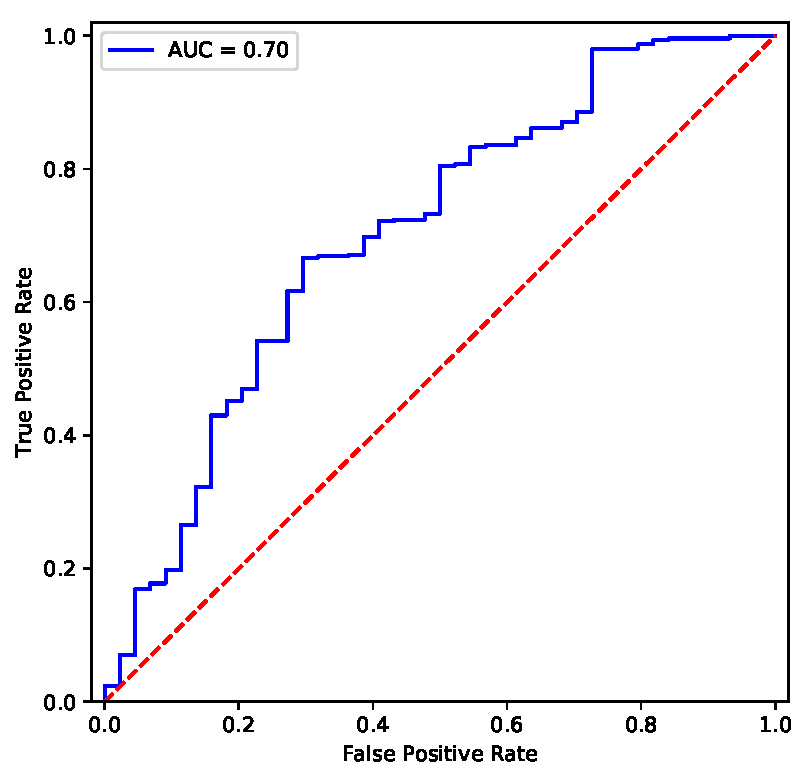
\includegraphics[width=3.2in]{ROC_Validation_on_Annotated_Corpus.pdf}\\
		\caption{ROC Curve, or the probability that $ P (\tau (e) > \tau (e \prime)) $, of the "place-of-birth" dataset}
		\label{pob_roc}
	\end{center}
\end{figure}

\begin{figure}[H]
	\begin{center}
		\includegraphics[width=3.2in]{grec_roc2.pdf}\\
		\caption{ROC Curve, or the probability that $ P (\tau (e) > \tau (e \prime)) $, of the "education-degree" dataset}
		\label{pob_roc2}
	\end{center}
\end{figure}



\newpage

\chapter{Conclusions and Recommendations}

\subsection{Conclusions}
This study was able to demonstrate the use of knowledge graphs and the cosine similarity measure for fact-checking. \\

In the first phase of the study, the use of metric closure in calculating truth values, weighed down with cosine similarity, was found out to be the more accurate algorithm over the three algorithms tested. It was able to classify the list of politicians into either Republican or Democrat accurately (having an area under the ROC curve of 0.72), and performed better than using ultrametric closure with TF-IDF + Cosine Similarity, and metric closure using only the generality of nodes (AUROC of 0.64 and 0.63, respectively).\\

The ultrametric closure was less accurate than its counterpart, metric closure. An educated guess would be that ultrametric closure is inherently inaccurate for fact-checking, since ultrametric closure would lead to a large distortion of the graph and discards other nodes in a path, except for the weakest link \cite{simas2015distance}. Metric closure, unlike its counterpart, imposes "built-in" penalties to the path, since it sums all the the distance weight in of every edge \cite{simas2015distance} (in the context of this study, the generality of the nodes are summed up, and weighed down using cosine similarity). This leads to more accurate results when determining how semantically related two entities are.\\

% PHASE 2 problems.
% - Good because it gives higher support for true statements.
% But the problem is, on some topics, it gives some false positives, because refer to my notes.
In the second phase of the study, the metric closure with TF-IDF + cosine similarity was used on factual data, on four topics. The probability that true statements have higher truth values than false statements were generally high on all four topics, and thus the fact checking method was able to discriminate between false and true statements accurately.\\

In the third phase, the fact checking of human fact checkers was compared to the computational fact checking method. This was done by using Google's Relation Extraction Corpus as the basis for human fact checkers. The scores given by human fact checkers were aggregated and then compared to the score given by the computational fact checking method. Rank order correlation coefficients were computed, specifically Spearman's $ \rho $ and Kendall's $ \tau $. Based on the results, there is a positive correlation between human fact checkers and the computational fact checking method. Additionally, the low p-values suggest that the correlation is statistically significant, rejecting the null hypothesis.\\

The results of this research is that the use of the metric closure in knowledge graphs, weighed down with cosine similarity, can increase the accuracy of fact checking. Although the results show that is a drawback when using cosine similarity: different statements having similar article text can lead to false positives, depending on how frequent each word in the vocabulary appears in all of the subjects and objects. However, the probability that a true statement has a higher truth value than false ones is still very high (see Table \ref{table_phase2}), thus making it feasible for computational fact checking, if modified in the future to overcome these drawbacks.


\subsection{Recommendations}

Despite the accuracy of fact checking found in the results of this study, there is still room for improvement in this field. The proponents would recommend the following:

\begin{enumerate}
	\item The proponents had utilized information from Wikipedia and Wikidata, but only extracted the article text and the generality (backlinks). There are plenty of meta-properties in Wikipedia/Wikidata that can be utilized to make the fact checking more specific and accurate.
	\item There is also room for improvement in the similarity measure: either an improved cosine similarity or another similarity measure that is more sensitive to the context of the statement being fact-checked.
	\item The computational fact checking method relies purely on the semantic similarity of the subject and the object, and discards the predicate, thus removing a significant extent of context and information. Future work can improve this study by putting more emphasis on the predicate part of a statement.
\end{enumerate}







\begin{appendices}
	\section{Ideological Classification Task}
	The following politicians were used for the ideological classification task:\\
\begin{table}[H]
	\tiny
	\begin{tabular}{|p{2in}|p{0.5in}||p{2in}|p{0.5in}|}
		
		\hline
		Politician & Party & Politician & Party\\ \hline
		Jo Bonner & Republican & Martha Roby & Republican\\ \hline
		Mike Rogers & Republican & Robert Aderholt & Republican\\ \hline
		Mo Brooks & Republican & Spencer Bachus & Republican\\ \hline
		Terri Sewell & Democrat & Paul Gosar & Republican\\ \hline
		Trent Franks & Republican & Ben Quayle & Republican\\ \hline
		Ed Pastor & Democrat & David Schweikert & Republican\\ \hline
		Jeff Flake & Republican & Raúl Grijalva & Democrat\\ \hline
		Gabrielle Giffords & Democrat & Ron Barber & Democrat\\ \hline
		Timothy Griffin & Republican & Steve Womack & Republican\\ \hline
		Mike Ross & Democrat & Wally Herger & Republican\\ \hline
		Dan Lungren & Republican & Tom McClintock & Republican\\ \hline
		Doris Matsui & Democrat & Lynn Woolsey & Democrat\\ \hline
		George Miller & Democrat & Nancy Pelosi & Democrat\\ \hline
		Barbara Lee & Democrat & John Garamendi & Democrat\\ \hline
		Jerry McNerney & Democrat & Jackie Speier & Democrat\\ \hline
		Pete Stark & Democrat & Anna Eshoo & Democrat\\ \hline
		Mike Honda & Democrat & Zoe Lofgren & Democrat\\ \hline
		Sam Farr & Democrat & Dennis Cardoza & Democrat\\ \hline
		Jeff Denham & Republican & Jim Costa & Democrat\\ \hline
		Devin Nunes & Republican & Lois Capps & Democrat\\ \hline
		Elton Gallegly & Republican & Howard McKeon & Republican\\ \hline
		David Dreier & Republican & Brad Sherman & Democrat\\ \hline
		Howard Berman & Democrat & Adam Schiff & Democrat\\ \hline
		Henry Waxman & Democrat & Xavier Becerra & Democrat\\ \hline
		Judy Chu & Democrat & Karen Bass & Democrat\\ \hline
		Lucille Roybal-Allard & Democrat & Maxine Waters & Democrat\\ \hline
		Jane Harman & Democrat & Janice Hahn & Democrat\\ \hline
		Laura Richardson & Democrat & Grace Napolitano & Democrat\\ \hline
		Linda Sanchez & Democrat & Ed Royce & Republican\\ \hline
		Jerry Lewis & Republican & Gary Miller & Republican\\ \hline
		Joe Baca & Democrat & Ken Calvert & Republican\\ \hline
		Mary Bono Mack & Republican & Dana Rohrabacher & Republican\\ \hline
		Loretta Sanchez & Democrat & Darrell Issa & Republican\\ \hline
		Brian Bilbray & Republican & Bob Filner & Democrat\\ \hline
		Duncan D. Hunter & Republican & Susan Davis & Democrat\\ \hline
		Diana DeGette & Democrat & Jared Polis & Democrat\\ \hline
		Scott Tipton & Republican & Cory Gardner & Republican\\ \hline
		Doug Lamborn & Republican & Mike Coffman & Republican\\ \hline
		Ed Perlmutter & Democrat & John Larson & Democrat\\ \hline
		Rosa DeLauro & Democrat & Jim Himes & Democrat\\ \hline
		Chris Murphy & Democrat & Corrine Brown & Democrat\\ \hline
		Ander Crenshaw & Republican & Rich Nugent & Republican\\ \hline
		Cliff Stearns & Republican & John Mica & Republican\\ \hline
		Daniel Webster & Republican & Gus Bilirakis & Republican\\ \hline
		Bill Young & Republican & Kathy Castor & Democrat\\ \hline
		Dennis Ross & Republican & Vern Buchanan & Republican\\ \hline
		Connie Mack & Republican & Bill Posey & Republican\\ \hline
		Frederica Wilson & Democrat & Ileana Ros-Lehtinen & Republican\\ \hline
		Ted Deutch & Democrat & Debbie Wasserman Schultz & Democrat\\ \hline
		Allen West (politician) & Republican & Alcee Hastings & Democrat\\ \hline
		Sandy Adams & Republican & David Rivera & Republican\\ \hline
		Jack Kingston & Republican & Sanford Bishop & Democrat\\ \hline
		Lynn Westmoreland & Republican & Hank Johnson & Democrat\\ \hline
		Rob Woodall & Republican & Austin Scott (politician) & Republican\\ \hline
		Tom Graves & Republican & Paul Broun & Republican\\ \hline
		Phil Gingrey & Republican & John Barrow (U.S. politician) & Democrat\\ \hline
		David Scott & Democrat & Mazie Hirono & Democrat\\ \hline
		Mike Simpson & Republican & Bobby Rush & Democrat\\ \hline
		Jesse Jackson Jr. & Democrat & Dan Lipinski & Democrat\\ \hline
		Luis Gutierrez & Democrat & Michael Quigley & Democrat\\ \hline
		Peter Roskam & Republican & Jan Schakowsky & Democrat\\ \hline
		Bob Dold & Republican & Adam Kinzinger & Republican\\ \hline
		Jerry Costello & Democrat & Judy Biggert & Republican\\ \hline
		Randy Hultgren & Republican & Don Manzullo & Republican\\ \hline
		Bobby Schilling & Republican & Aaron Schock & Republican\\ \hline
		John Shimkus & Republican & Pete Visclosky & Democrat\\ \hline
		Joe Donnelly & Democrat & Marlin Stutzman & Republican\\ \hline
		Todd Rokita & Republican & Dan Burton & Republican\\ \hline
		Mike Pence & Republican & Larry Bucshon & Republican\\ \hline
		Todd Young & Republican & Bruce Braley & Democrat\\ \hline


	\end{tabular}
\end{table}


\begin{table}[H]
	\tiny
	\begin{tabular}{|p{2in}|p{0.5in}||p{2in}|p{0.5in}|}
		\hline
		Politician & Party & Politician & Party\\ \hline
		David Loebsack & Democrat & Leonard Boswell & Democrat\\ \hline
		Steve King & Republican & Tim Huelskamp & Republican\\ \hline
		Lynn Jenkins & Republican & Kevin Yoder & Republican\\ \hline
		Mike Pompeo & Republican & Ed Whitfield & Republican\\ \hline
		Brett Guthrie & Republican & John Yarmuth & Democrat\\ \hline
		Geoff Davis & Republican & Hal Rogers & Republican\\ \hline
		Ben Chandler & Democrat & Steve Scalise & Republican\\ \hline
		Cedric Richmond & Democrat & Jeff Landry & Republican\\ \hline
		John Fleming (American politician) & Republican & Rodney Alexander & Republican\\ \hline
		Bill Cassidy & Republican & Charles Boustany & Republican\\ \hline
		Chellie Pingree & Democrat & Mike Michaud & Democrat\\ \hline
		Andy Harris (politician) & Republican & Dutch Ruppersberger & Democrat\\ \hline
		John Sarbanes & Democrat & Donna Edwards & Democrat\\ \hline
		Steny Hoyer & Democrat & Roscoe Bartlett & Republican\\ \hline
		Elijah Cummings & Democrat & Chris Van Hollen & Democrat\\ \hline
		John Olver & Democrat & Barney Frank & Democrat\\ \hline
		Niki Tsongas & Democrat & John F. Tierney & Democrat\\ \hline
		Ed Markey & Democrat & Mike Capuano & Democrat\\ \hline
		William R. Keating & Democrat & Dan Benishek & Republican\\ \hline
		Bill Huizenga & Republican & Jeff Sessions & Republican\\ \hline
		Richard Shelby & Republican & Mark Begich & Democrat\\ \hline
		Lisa Murkowski & Republican & Jon Kyl & Republican\\ \hline
		John McCain & Republican & Mark Pryor & Democrat\\ \hline
		John Boozman & Republican & Dianne Feinstein & Democrat\\ \hline
		Barbara Boxer & Democrat & Mark Udall & Democrat\\ \hline
		Michael Bennet & Democrat & Richard Blumenthal & Democrat\\ \hline
		Tom Carper & Democrat & Chris Coons & Democrat\\ \hline
		Bill Nelson (politician) & Democrat & Marco Rubio & Republican\\ \hline
		Saxby Chambliss & Republican & Johnny Isakson & Republican\\ \hline
		Daniel Akaka & Democrat & Daniel Inouye & Democrat\\ \hline
		Brian Schatz & Democrat & Jim Risch & Republican\\ \hline
		Mike Crapo & Republican & Dick Durbin & Democrat\\ \hline
		Mark Kirk & Republican & Richard Lugar & Republican\\ \hline
		Dan Coats & Republican & Tom Harkin & Democrat\\ \hline
		Chuck Grassley & Republican & Rand Paul & Republican\\ \hline
		Mitch McConnell & Republican & Mary Landrieu & Democrat\\ \hline
		David Vitter & Republican & Olympia Snowe & Republican\\ \hline
		Susan Collins & Republican & Ben Cardin & Democrat\\ \hline
		Barbara Mikulski & Democrat & Scott Brown (politician) & Republican\\ \hline
		John Kerry & Democrat & Debbie Stabenow & Democrat\\ \hline
		Carl Levin & Democrat & Amy Klobuchar & Democrat\\ \hline
		Al Franken & Democrat & Roger Wicker & Republican\\ \hline
		Thad Cochran & Republican & Claire McCaskill & Democrat\\ \hline
		Roy Blunt & Republican & Jon Tester & Democrat\\ \hline
		Max Baucus & Democrat & Ben Nelson & Democrat\\ \hline
		Mike Johanns & Republican & John Ensign & Republican\\ \hline
		Dean Heller & Republican & Harry Reid & Democrat\\ \hline
		Jeanne Shaheen & Democrat & Kelly Ayotte & Republican\\ \hline
		Bob Menendez & Democrat & Frank Lautenberg & Democrat\\ \hline
		Jeff Bingaman & Democrat & Tom Udall & Democrat\\ \hline
		Kirsten Gillibrand & Democrat & Charles Schumer & Democrat\\ \hline
		Kay Hagan & Democrat & Richard Burr & Republican\\ \hline
		Kent Conrad & Democrat & John Hoeven & Republican\\ \hline
		Sherrod Brown & Democrat & Rob Portman & Republican\\ \hline
		Jim Inhofe & Republican & Tom Coburn & Republican\\ \hline
		Jeff Merkley & Democrat & Ron Wyden & Democrat\\ \hline
		Pat Toomey & Republican & Sheldon Whitehouse & Democrat\\ \hline
		Jack Reed (Rhode Island politician) & Democrat & Lindsey Graham & Republican\\ \hline
		Jim DeMint & Republican & Tim Scott & Republican\\ \hline
		John Thune & Republican & Bob Corker & Republican\\ \hline
		Lamar Alexander & Republican & Kay Bailey Hutchison & Republican\\ \hline
		John Cornyn & Republican & Orrin Hatch & Republican\\ \hline
		Mike Lee (U.S. politician) & Republican & Patrick Leahy & Democrat\\ \hline
		Jim Webb & Democrat & Mark Warner & Democrat\\ \hline
		Maria Cantwell & Democrat & Patty Murray & Democrat\\ \hline
		Joe Manchin & Democrat & Jay Rockefeller & Democrat\\ \hline
		Herb Kohl & Democrat & John Barrasso & Republican\\ \hline
	\end{tabular}
\end{table}

The list of ideologies used in the first phase:\\
Anarchism; Antisemitism; Capitalism; Christianity; Communism; Conservatism; Democracy; Fascism; Feminism; Islamophobia; Left-wing politics; Liberalism; Marxism; Nationalism; Neo-Nazism; Protestantism; Right-wing politics; Secularism; Socialism; White supremacy

\newpage
\section{Validation on Annotated Data}
Data gathered for the second phase:
\subsubsection{US President - Spouses}
\begin{table}[H]
	\begin{center}
		\begin{tabular}{|p{2in}|p{2in}|} \hline 
			US President & Spouse \\ \hline 
			Woodrow Wilson & Edith Wilson \\ \hline 
			Warren G. Harding & Florence Harding \\ \hline 
			Calvin Coolidge & Grace Coolidge \\ \hline 
			Herbert Hoover & Lou Henry Hoover \\ \hline 
			Franklin D. Roosevelt & Eleanor Roosevelt \\ \hline 
			Harry S. Truman & Bess Truman \\ \hline 
			Dwight D. Eisenhower & Mamie Eisenhower \\ \hline 
			John F. Kennedy & Jacqueline Kennedy Onassis \\ \hline 
			Lyndon B. Johnson & Lady Bird Johnson \\ \hline 
			Richard Nixon & Pat Nixon \\ \hline 
			Gerald Ford & Betty Ford \\ \hline 
			Jimmy Carter & Rosalynn Carter \\ \hline 
			Ronald Reagan & Nancy Reagan \\ \hline 
			George H. W. Bush & Barbara Bush \\ \hline 
			Bill Clinton & Hillary Clinton \\ \hline 
			George W. Bush & Laura Bush \\ \hline 
			Barack Obama & Michelle Obama \\ \hline 
		\end{tabular}
	\end{center}
\end{table}

\subsection{Country - Capitals}
\begin{table}[H]
	\begin{center}
		\begin{tabular}{|p{3in}|p{3in}|} \hline 
			Country & Capital \\ \hline 
			Eritrea & Asmara \\ \hline 
			Ghana & Accra \\ \hline 
			Malaysia & Kuala Lumpur \\ \hline 
			Mozambique & Maputo \\ \hline 
			Sudan & Khartoum \\ \hline 
			Zimbabwe & Harare \\ \hline 
			Philippines & Manila \\ \hline 
			Saudi Arabia & Riyadh \\ \hline 
			Uzbekistan & Tashkent \\ \hline 
			Vietnam & Hanoi \\ \hline 
			Croatia & Zagreb \\ \hline 
			Italy & Rome \\ \hline 
			Romania & Bucharest \\ \hline 
			Spain & Madrid \\ \hline 
			Switzerland & Bern \\ \hline 
			Canada & Ottawa \\ \hline 
			Haiti & Port-au-Prince \\ \hline 
			Kingdom of the Netherlands & Amsterdam \\ \hline 
			Saint Vincent and the Grenadines & Kingstown \\ \hline 
			United States & Washington D.C. \\ \hline 
			Australia & Canberra \\ \hline 
			Kiribati & South Tarawa \\ \hline 
			New Zealand & Wellington \\ \hline 
			Solomon Islands & Honiara \\ \hline 
			Vanuatu & Port Vila \\ \hline 
			Bolivia & Sucre \\ \hline 
			Ecuador & Quito \\ \hline 
			Guyana & Georgetown Guyana \\ \hline 
			Suriname & Paramaribo \\ \hline 
			Venezuela & Caracas \\ \hline 
		\end{tabular}
	\end{center}
\end{table}

\subsection{Movie - Directors}
\begin{table}[H]
	\begin{center}
		\begin{tabular}{|p{3in}|p{3in}|} \hline 
			Director & Movie \\ \hline 
			Kramer vs Kramer & Robert Benton \\ \hline 
			Ordinary People & Robert Redford \\ \hline 
			Reds (film) & Warren Beatty \\ \hline 
			Gandhi (film) & Richard Attenborough \\ \hline 
			Terms of Endearment & James L. Brooks \\ \hline 
			Amadeus (film) & Milo\v{s} Forman \\ \hline 
			Out of Africa (film) & Sydney Pollack \\ \hline 
			Platoon (film) & Oliver Stone \\ \hline 
			The Last Emperor & Bernardo Bertolucci \\ \hline 
			Rain Man & Barry Levinson \\ \hline 
			Dances with Wolves & Kevin Costner \\ \hline 
			The Silence of the Lambs (film) & Jonathan Demme \\ \hline 
			Unforgiven & Clint Eastwood \\ \hline 
			Forrest Gump & Robert Zemeckis \\ \hline 
			Braveheart & Mel Gibson \\ \hline 
			The English Patient (film) & Anthony Minghella \\ \hline 
			Titanic (1997 film) & James Cameron \\ \hline 
			Saving Private Ryan & Steven Spielberg \\ \hline 
			American Beauty (1999 film) & Sam Mendes \\ \hline 
			Traffic (2000 film) & Steven Soderbergh \\ \hline 
			A Beautiful Mind (film) & Ron Howard \\ \hline 
			The Pianist (2002 film) & Roman Polanski \\ \hline 
			Brokeback Mountain & Ang Lee \\ \hline 
			The Departed & Martin Scorsese \\ \hline 
			No Country for Old Men (film) & Joel and Ethan Coen \\ \hline 
			Slumdog Millionaire & Danny Boyle \\ \hline 
			The Hurt Locker & Kathryn Bigelow \\ \hline 
			The Artist (film) & Michel Hazanavicius \\ \hline 
			Gravity (2013 film) & Alfonso Cuar\'{o}n \\ \hline 
		\end{tabular}
	\end{center}
\end{table}

\subsection{US State - Capitals}
\begin{table}[H]
	\begin{center}
		\begin{tabular}{|p{3in}|p{3in}|} \hline 
			State & Capital \\ \hline 
			Illinois & Springfield, Illinois \\ \hline 
			Indiana & Indianapolis \\ \hline 
			Iowa & Des Moines, Iowa \\ \hline 
			Kansas & Topeka, Kansas \\ \hline 
			Michigan & Lansing, Michigan \\ \hline 
			Minnesota & Saint Paul, Minnesota \\ \hline 
			Missouri & Jefferson City, Missouri \\ \hline 
			Pennsylvania & Harrisburg, Pennsylvania \\ \hline 
			Rhode Island & Providence, Rhode Island \\ \hline 
			Vermont & Montpelier, Vermont \\ \hline 
			Alabama & Montgomery, Alabama \\ \hline 
			Arkansas & Little Rock, Arkansas \\ \hline 
			Delaware & Dover, Delaware \\ \hline 
			Florida & Tallahassee, Florida \\ \hline 
			Louisiana & Baton Rouge, Louisiana \\ \hline 
			Maryland & Annapolis, Maryland \\ \hline 
			Mississippi & Jackson, Mississippi \\ \hline 
			North Carolina & Raleigh, North Carolina \\ \hline 
			Oklahoma & Oklahoma City \\ \hline 
			Tennessee & Nashville, Tennessee \\ \hline 
			Texas & Austin, Texas \\ \hline 
			Arizona & Phoenix, Arizona \\ \hline 
			California & Sacramento, California \\ \hline 
			Nevada & Carson City, Nevada \\ \hline 
			New Mexico & Santa Fe, New Mexico \\ \hline 
			Oregon & Salem, Oregon \\ \hline 
			Utah & Salt Lake City, Utah \\ \hline 
			Wyoming & Cheyenne, Wyoming \\ \hline 
		\end{tabular}
	\end{center}
\end{table}


\end{appendices}
































\bibliographystyle{acm}
\bibliography{references}

\end{document}

